\section{Data}\label{data}

The data are French EU-SILC, collection year 2016, with income reference year 2015. Taxes, benefits and disposable income are computed by EUROMOD \citep{sutherlandfigari2013} under the French 2015 policy system, which is the system in force over the income reference period. We use the same three dates consistently: the survey is collected in 2016, incomes refer to 2015, and the simulated policy system is 2015.

\subsection{The estimation samples}\label{the-estimation-samples}

\Needspace*{12\baselineskip}\small\setlength{\tabcolsep}{3pt}\begin{longtable}[]{@{}
  >{\raggedright\arraybackslash}p{(\linewidth - 4\tabcolsep) * \real{0.3333}}
  >{\raggedright\arraybackslash}p{(\linewidth - 4\tabcolsep) * \real{0.3333}}
  >{\raggedright\arraybackslash}p{(\linewidth - 4\tabcolsep) * \real{0.3333}}@{}}
\caption{Sample construction. Unweighted households remaining after each screen, from the France 2016 EUROMOD input file to the two estimation samples. Rows are sequential; the counts are read from the frame records and are not reconstructed by subtraction.}\tabularnewline
\toprule\noalign{}
\begin{minipage}[b]{\linewidth}\raggedright
Screen
\end{minipage} & \begin{minipage}[b]{\linewidth}\raggedright
Single-adult
\end{minipage} & \begin{minipage}[b]{\linewidth}\raggedright
Couple
\end{minipage} \\
\midrule\noalign{}
\endfirsthead
\toprule\noalign{}
\begin{minipage}[b]{\linewidth}\raggedright
Screen
\end{minipage} & \begin{minipage}[b]{\linewidth}\raggedright
Single-adult
\end{minipage} & \begin{minipage}[b]{\linewidth}\raggedright
Couple
\end{minipage} \\
\midrule\noalign{}
\endhead
\bottomrule\noalign{}
\endlastfoot
the raw France 2016 input file & 4,038 & 5,965 \\
one- or two-adult households (composition screen) & 4,038 & 5,965 \\
every adult aged 20 to 60 & 2,131 & 3,662 \\
no adult still in education & 2,036 & 3,521 \\
no old-age, disability or survivor pension receipt & 1,755 & 3,218 \\
labour status in scope & 1,598 & 2,412 \\
no other employable or earning member & 1,564 & 2,323 \\
observed hours and wage inside the calibrated support & 1,555 & 2,275 \\
hours outside {[}5,70{]} or unsupported military occupation (ISCO 0) on an employed decider & 1,543 & 2,223 \\
observed chosen alternative priced at non-positive disposable consumption & 1,540 & 2,223 \\
\textbf{Estimation sample} & \textbf{1,540} & \textbf{2,223} \\
\end{longtable}

The screens are of three kinds and it is worth separating them. The first two define the decision unit: the household must contain either one unpartnered adult or two mutually linked adults of opposite sex, and every decider must be between twenty and sixty. This is the largest exclusion and it is structural. Multi-generational households, flat-shares, adult children living with parents and same-sex couples are outside the estimated population, and no result extends to them. Because the age screen binds on both spouses, it removes proportionally more couples than singles.

The second kind removes households for whom the model does not define an offer set: adults in full-time education, households receiving an old-age, disability or survivor pension, and deciders whose labour-market status lies outside employment, unemployment and inactivity. Together with the pension screen this is why the surviving employment rate is high. The employment share below should be read as a share among people for whom working is a live option, not as a French employment rate.

The third kind is support. An employed decider's observed hours must lie in the closed interval \([5, 70]\) hours per week and the delivered hourly wage in \([2, 590]\) euros per hour, because those are the boundaries of the supports the opportunity densities are defined on. An observed occupation must map into the four modelled groups; ISCO 0, the armed forces, does not, and the resulting exclusion is \emph{unsupported} occupation, not missing occupation. Three single-adult households whose own observed job prices to non-positive disposable consumption are removed, because the log-consumption term is undefined at their observed choice; non-positive \emph{simulated} alternatives are not a reason to drop a household, and are instead excluded from that household's choice domain.

\Needspace*{12\baselineskip}\small\setlength{\tabcolsep}{3pt}\begin{longtable}[]{@{}
  >{\raggedright\arraybackslash}p{(\linewidth - 4\tabcolsep) * \real{0.3333}}
  >{\raggedright\arraybackslash}p{(\linewidth - 4\tabcolsep) * \real{0.3333}}
  >{\raggedright\arraybackslash}p{(\linewidth - 4\tabcolsep) * \real{0.3333}}@{}}
\caption{The four occupation groups. ISCO-08 major groups are aggregated into four modelled groups; group 1 is the omitted reference in the estimated occupation block. This is a research aggregation adopted for this paper, not an ILO classification. ISCO 0, the armed forces, has no modelled alternative and is a sample screen; that is unsupported occupation, not missing occupation.}\tabularnewline
\toprule\noalign{}
\begin{minipage}[b]{\linewidth}\raggedright
Model group
\end{minipage} & \begin{minipage}[b]{\linewidth}\raggedright
ISCO-08 major groups
\end{minipage} & \begin{minipage}[b]{\linewidth}\raggedright
Description
\end{minipage} \\
\midrule\noalign{}
\endfirsthead
\toprule\noalign{}
\begin{minipage}[b]{\linewidth}\raggedright
Model group
\end{minipage} & \begin{minipage}[b]{\linewidth}\raggedright
ISCO-08 major groups
\end{minipage} & \begin{minipage}[b]{\linewidth}\raggedright
Description
\end{minipage} \\
\midrule\noalign{}
\endhead
\bottomrule\noalign{}
\endlastfoot
1 (reference) & 6--9 & Skilled agricultural, craft, plant and machine operators, and elementary occupations \\
2 & 5 & Service and sales workers \\
3 & 4 & Clerical support workers \\
4 & 1--3 & Managers, professionals, technicians and associate professionals \\
\end{longtable}

\subsection{What the households look like}\label{what-the-households-look-like}

\Needspace*{12\baselineskip}\small\setlength{\tabcolsep}{3pt}\begin{longtable}[]{@{}>{\RaggedRight\arraybackslash}p{0.2500\linewidth}>{\RaggedRight\arraybackslash}p{0.2247\linewidth}>{\RaggedRight\arraybackslash}p{0.2247\linewidth}>{\RaggedRight\arraybackslash}p{0.2247\linewidth}@{}}
\caption{Descriptive means on the estimation samples. Weighted by the household cross-sectional weight; one row per household, with spouse-specific variables carried on the household row. Hours and wages are conditional on employment. These are observed inputs, not model predictions.}\tabularnewline
\toprule\noalign{}
Measure & Single-adult decider & Couple man & Couple woman \\
\midrule\noalign{}
\endfirsthead
\toprule\noalign{}
Measure & Single-adult decider & Couple man & Couple woman \\
\midrule\noalign{}
\endhead
\bottomrule\noalign{}
\endlastfoot
Age (years) & 41.1 & 39.8 & 37.8 \\
Children under 20 & -- & -- & -- \\
Usual weekly hours, employed & 37.6 & 41.1 & 35.8 \\
Delivered hourly wage, employed (EUR/hour) & -- & -- & -- \\
Households (unweighted) & 1,540 & 2,223 & \\
\end{longtable}

\begin{figure}[H]
\centering
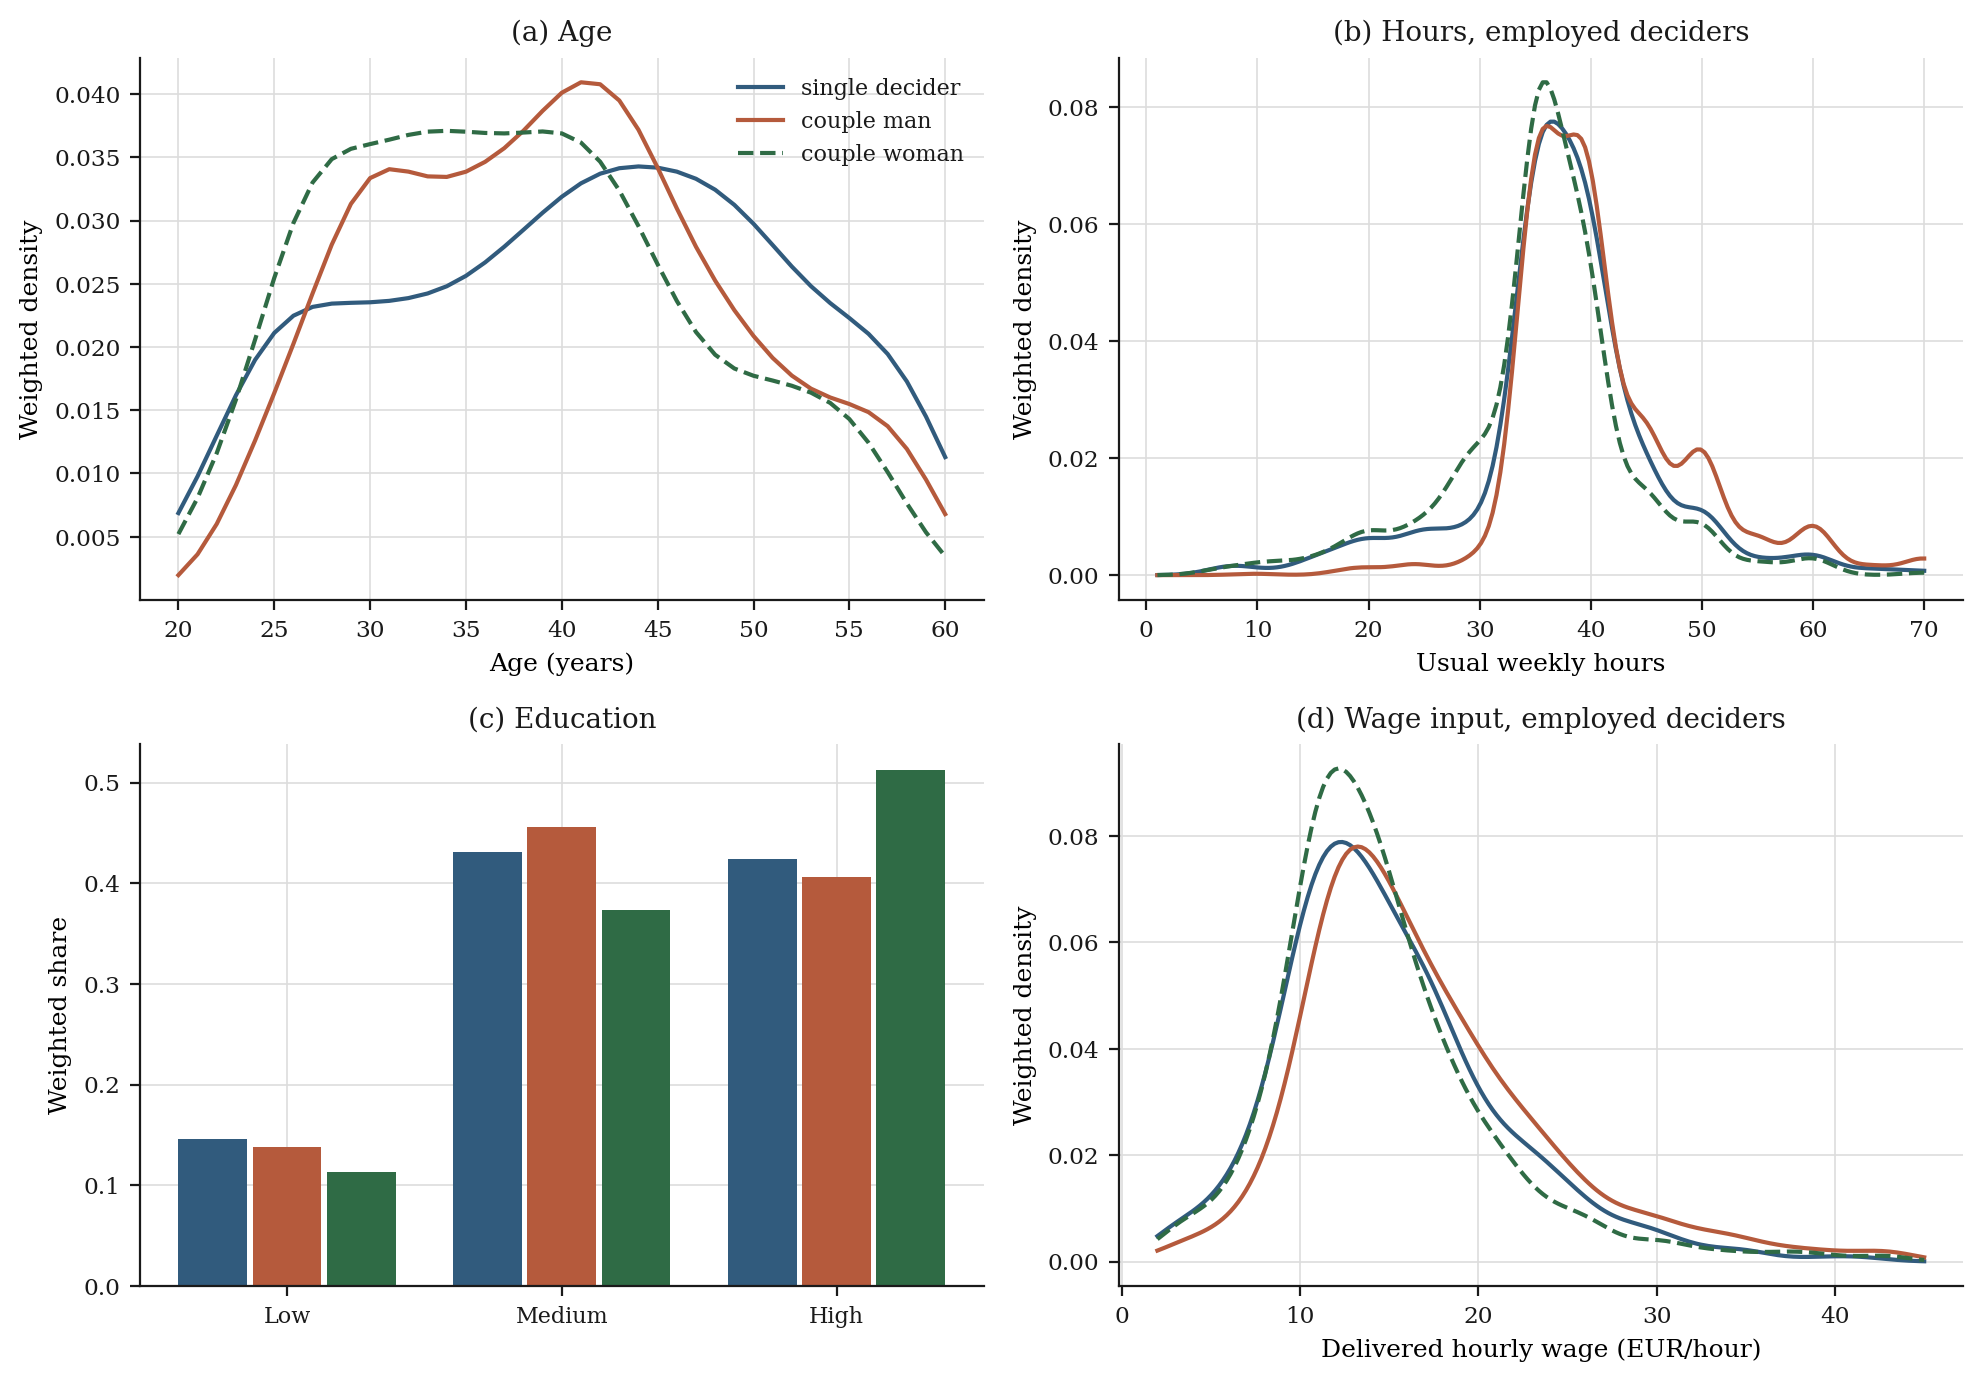
\includegraphics[width=0.95\linewidth,height=\textheight,keepaspectratio,alt={Weighted distributions on the estimation samples: age, usual weekly hours among employed deciders, education, and the delivered hourly wage input. Observed inputs, not model predictions.}]{figures/v5/figV08_data_panel.png}
\caption{Weighted distributions on the estimation samples: age, usual weekly hours among employed deciders, education, and the delivered hourly wage input. Observed inputs, not model predictions.}
\end{figure}

Education is the three-level ISCED grouping, with the medium level as the omitted reference in the wage equation. Potential experience is years since leaving education, entering the wage equation in units of 20 years, with the square recomputed after scaling rather than carried forward. A child is any resident household member under 20, counted without a parent link. Age enters preferences centred on the sample mean decider age and divided by 10 years.

\Needspace*{12\baselineskip}\small\setlength{\tabcolsep}{3pt}\begin{longtable}[]{@{}>{\RaggedRight\arraybackslash}p{0.2500\linewidth}>{\RaggedRight\arraybackslash}p{0.1650\linewidth}>{\RaggedRight\arraybackslash}p{0.1650\linewidth}>{\RaggedRight\arraybackslash}p{0.1650\linewidth}>{\RaggedRight\arraybackslash}p{0.1650\linewidth}@{}}
\caption{Observed joint participation regimes among the 2,223 estimated couple households. These are joint regimes, not two spouse marginals.}\tabularnewline
\toprule\noalign{}
Regime & Meaning & Weighted share & Mean hours, man & Mean hours, woman \\
\midrule\noalign{}
\endfirsthead
\toprule\noalign{}
Regime & Meaning & Weighted share & Mean hours, man & Mean hours, woman \\
\midrule\noalign{}
\endhead
\bottomrule\noalign{}
\endlastfoot
BB & both spouses employed & 0.8435 & 41.0 & 35.9 \\
MO & man employed, woman not employed & 0.0796 & 41.5 & 0.0 \\
WO & woman employed, man not employed & 0.0547 & 0.0 & 35.0 \\
NN & neither spouse employed & 0.0222 & 0.0 & 0.0 \\
\end{longtable}

\subsection{The household budget}\label{the-household-budget}

For a given work arrangement the tax-benefit model is given the implied gross labour inputs, weekly hours, hourly wage, and earnings split at the thirty-five hour threshold, together with the household's non-labour inputs and roster, and returns disposable income. Only deciders receive counterfactual overrides; other members keep their baseline values. The accounting identity linking original income, benefits, taxes and social contributions to disposable income holds to machine precision at both the person and the household-alternative level, before and after the benefit take-up adjustment. Disposable income is summed over all resident members of the household.

\begin{figure}[H]
\centering
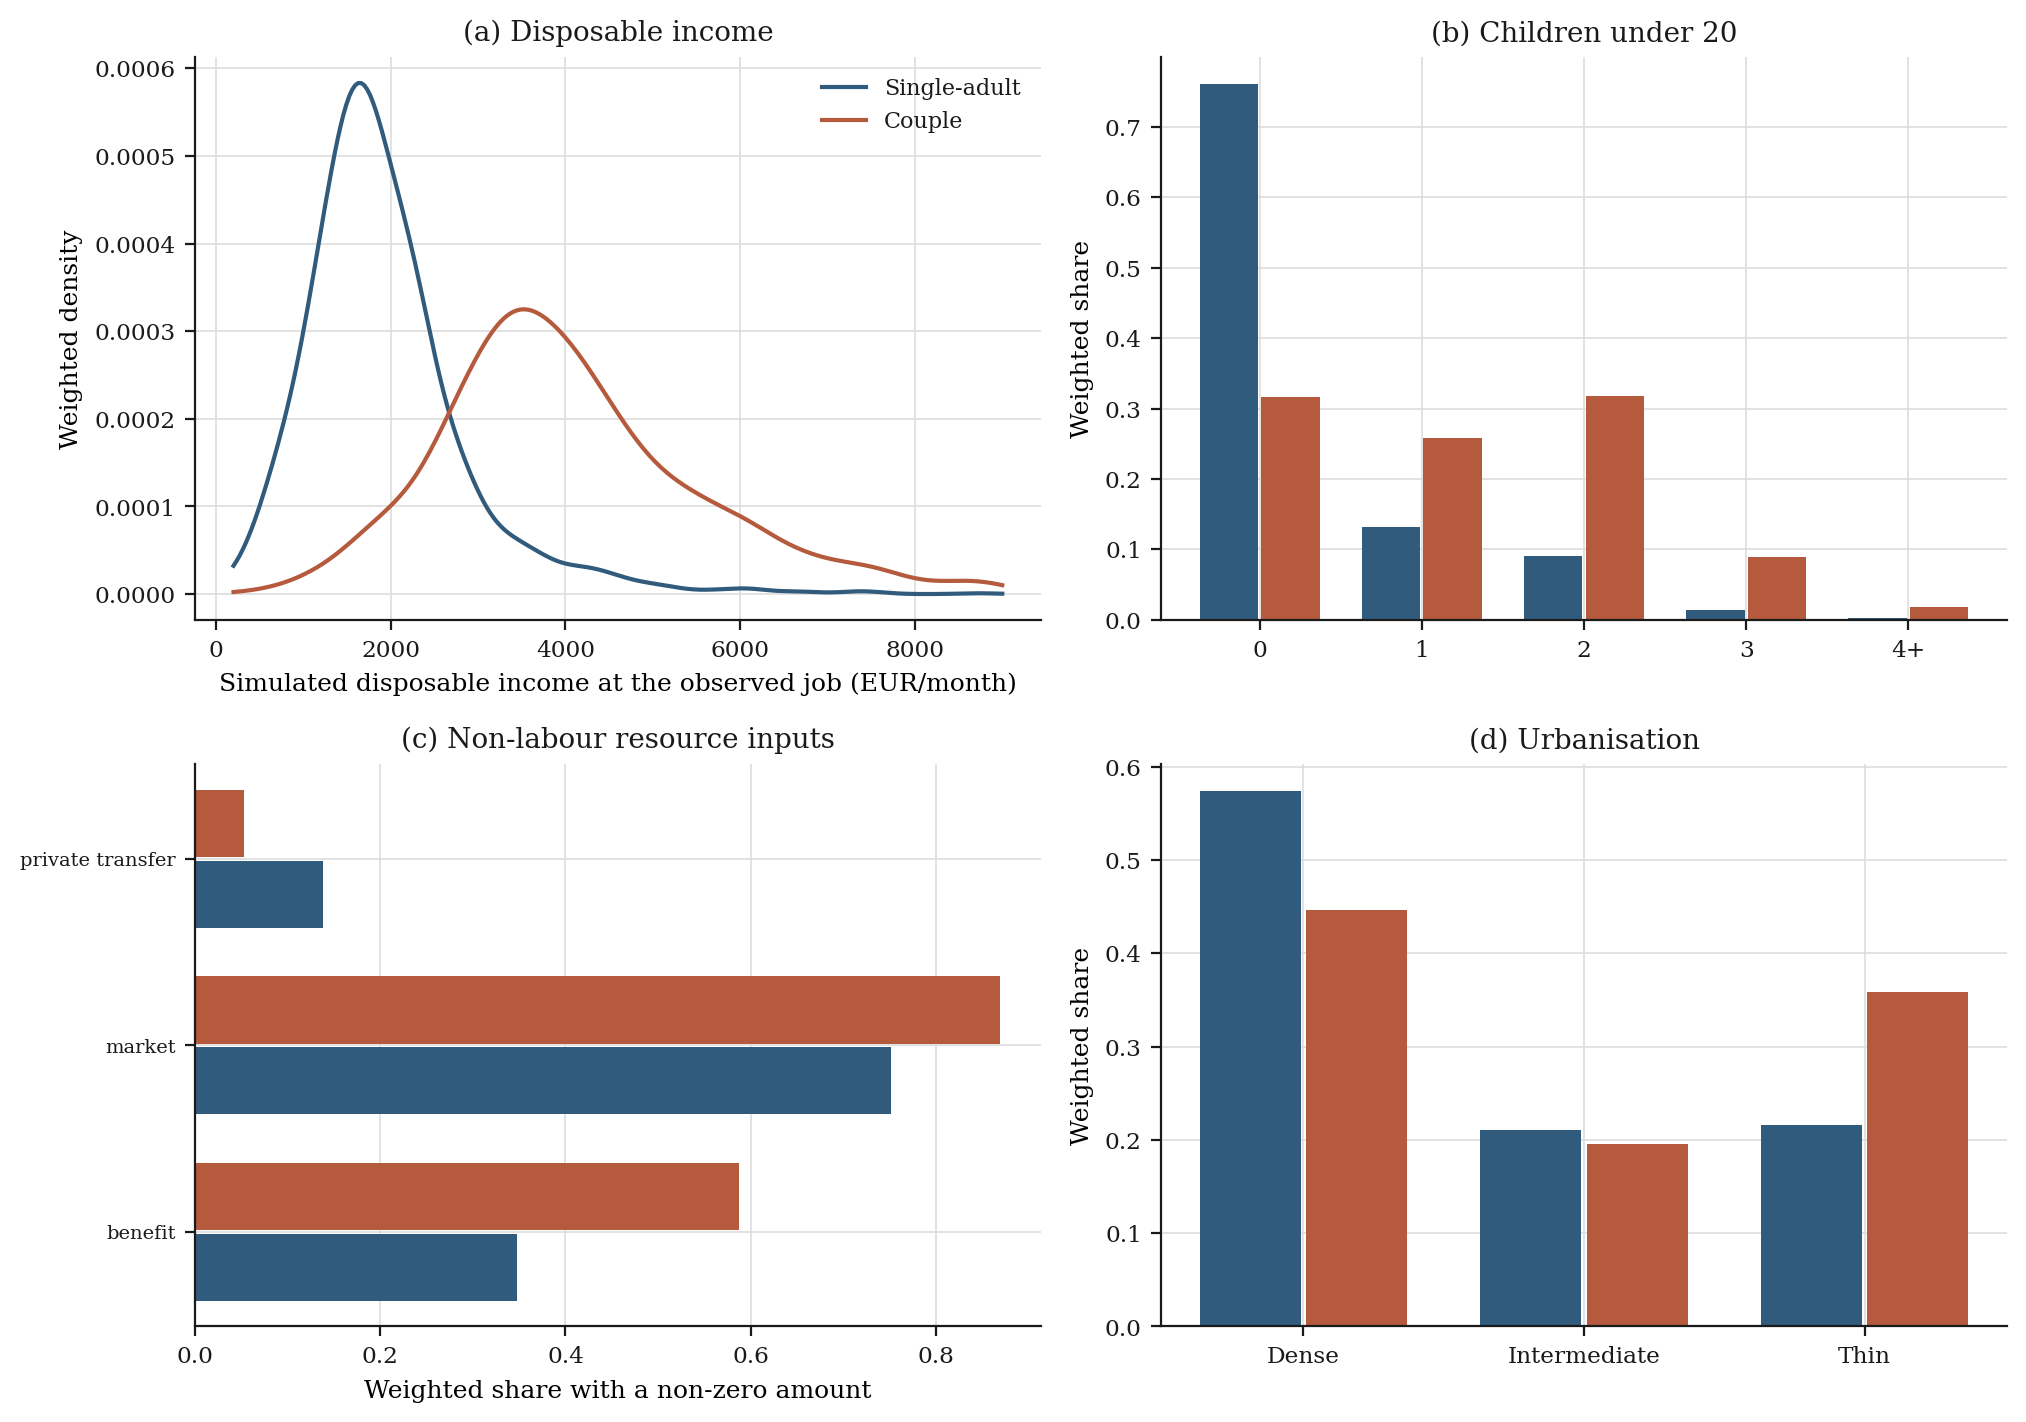
\includegraphics[width=0.95\linewidth,height=\textheight,keepaspectratio,alt={Weighted distributions on the estimation samples: simulated disposable income at the observed job, children under twenty, the incidence of non-labour budget inputs by family, and urbanisation. Panel (a) is a tax-benefit output evaluated at the observed choice; panel (c) reports inputs to that calculation. The two are never added, and stocks are never summed with monthly flows.}]{figures/v5/figV09_resources_panel.png}
\caption{Weighted distributions on the estimation samples: simulated disposable income at the observed job, children under twenty, the incidence of non-labour budget inputs by family, and urbanisation. Panel (a) is a tax-benefit output evaluated at the observed choice; panel (c) reports inputs to that calculation. The two are never added, and stocks are never summed with monthly flows.}
\end{figure}

Panel (c) of the figure reports the \emph{incidence} of non-labour budget inputs by family, not a cash total. Some of these are stocks, some are annual flows and some are monthly; they are inputs to the tax-benefit calculation and are not added together into one income concept. The pension family is empty by construction, because pension receipt is a sample screen. Panel (a) reports the tax-benefit \emph{output} at the observed job, which is an object of a different kind and is never added to panel (c).

Local labour-market conditions enter through a group unemployment measure, a population-weighted exposure index for the decider's region and age-education cell, stored as a fraction and entering the employment index multiplied by 10. Regional and urbanisation variation supports the access specification conditional on the exclusion restriction and the functional form; it does not by itself identify access, and no causal effect of geography is claimed anywhere in this paper.

